\documentclass{beamer}

% Frame Number
\setbeamertemplate{footline}[frame number]

% Input Encoding
\usepackage[utf8]{inputenc}

% PDF Bookmarks
\usepackage{url}
\usepackage{hyperref} 
\hypersetup{colorlinks}
\hypersetup{bookmarksopen}
\hypersetup{bookmarksnumbered}
\hypersetup{citecolor=blue}
\hypersetup{urlcolor=blue}
\hypersetup{linkcolor=blue}

% Spacing
\usepackage{xspace}

% Figures
\usepackage{graphicx}
\graphicspath{{../../img/}}
\usepackage{subcaption}

% Tables
\usepackage{booktabs}

% Strike Through
\usepackage{ulem}

% Code Snippet 
\usepackage{listings}
\lstset{
  belowcaptionskip=1\baselineskip,
  breaklines=true,
  frame=L,
  xleftmargin=\parindent,
  numbers=left,
  stepnumber=2,
  language=C,
  tabsize=2,
  showstringspaces=false,
  basicstyle=\footnotesize\ttfamily,
  keywordstyle=\bfseries\color{blue},
  commentstyle=\itshape\color{gray},
  identifierstyle=\bfseries\color{black},
  stringstyle=\bfseries\color{purple},
}

% Title
\title[Nanvix]{%
	\textbf{%
		The Nanvix Operating System\\
		\small{Buffer Pre-Fetching}
	}
}

% Authors
\author[Pedro H. Penna]{%
	Pedro H. Penna%
}

% Affiliations
\institute{
	\url{pedrohenriquepenna@gmail.com}
}

% Short-Hands
\newcommand{\ie}{\textit{ie.\xspace}}

\begin{document}

\frame{\titlepage}

\section{Background on I/O}

	\begin{frame}
	\frametitle{Background}
	\framesubtitle{Motivation}
		\begin{itemize}
		\setlength\itemsep{1.5em}
			\uncover<1->{
				\item User applications communicate
				\begin{itemize}
				\setlength\itemsep{0.5em}
					\item Keyboard
					\item Display
					\item Hard-Disks
				\end{itemize}
			}
			\uncover<2->{
				\item What if applications perform too much I/O?
			}
				\begin{itemize}
				\uncover<3->{
					\item Poor performance
				}
				\uncover<4->{
					\item Solution: relying caching
				}
				\end{itemize}
		\end{itemize}
	\end{frame}

	\begin{frame}
	\frametitle{Background}
	\framesubtitle{The Buffer Cache}
		\begin{itemize}
		\setlength\itemsep{1.5em}
			\uncover<1->{
				\item In-memory cache for disk-blocks
			}
			\uncover<2->{
				\item Keep most accessed data in memory
			}
			\uncover<3->{
				\item Asynchronous write data to disk
			}
			\uncover<4->{
				\item Pre-fetch disk block that will be used soon
			}
			\uncover<5->{
				\item Further abstracts the underlying device
			}
		\end{itemize}
	\end{frame}

\section{Buffer Cache in Nanvix}

	\begin{frame}
	\frametitle{Buffer Cache in Nanvix}
	\framesubtitle{The Buffer Cache}
		\begin{itemize}
		\setlength\itemsep{1.5em}
			\uncover<1->{
				\item LRU replacement policy
			}
			\uncover<2->{
				\item Asynchronous buffer write
			}
			\uncover<3->{
				\item No load control
			}
			\uncover<4->{
				\item No buffer pre-fetching
			}
		\end{itemize}
	\end{frame}

	\begin{frame}
	\frametitle{Buffer Cache in Nanvix}
	\framesubtitle{Buffer Cache Structure}
		\begin{figure}
			\centering
			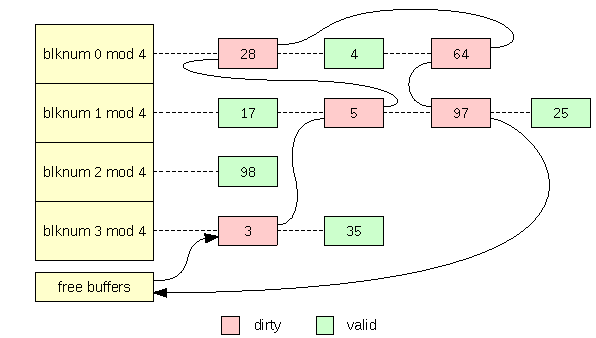
\includegraphics[width=0.9\linewidth]{buffer-cache}
			\caption{Buffer cache structure.}
		\end{figure}
	\end{frame}

	\begin{frame}
	\frametitle{Buffer Cache in Nanvix}
	\framesubtitle{I/O Software Stack}
		\begin{figure}
			\centering
			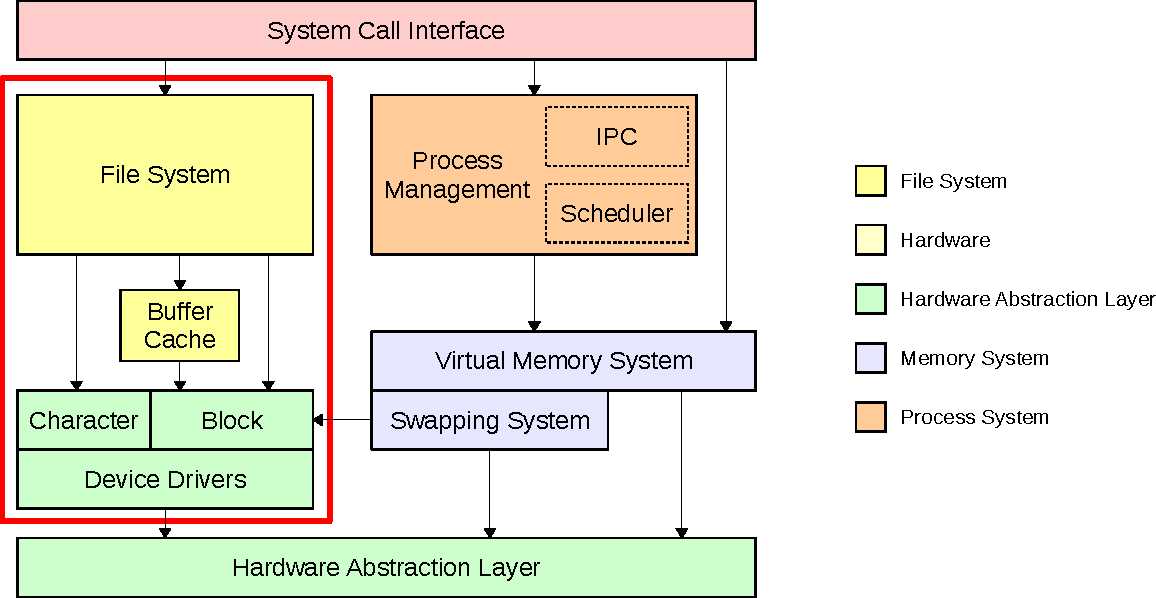
\includegraphics[width=0.9\linewidth]{io-software-stack}
			\caption{IO software stack in Nanvix.}
		\end{figure}
	\end{frame}

	\begin{frame}
	\frametitle{Buffer Cache in Nanvix}
	\framesubtitle{Current Implementation}
		\begin{itemize}
		\setlength\itemsep{1.0em}
			\uncover<1->{
				\item Read System Call -- \texttt{sys\_read()}
				\begin{itemize}
				\setlength\itemsep{0.5em}
					\item \texttt{src/kernel/sys/read.c}
				\end{itemize}
			}
			\uncover<2->{
				\item File Read -- \texttt{file\_read()}
				\begin{itemize}
				\setlength\itemsep{0.5em}
					\item \texttt{src/kernel/fs/file.c}
				\end{itemize}
			}
			\uncover<3->{
				\item Buffer Cache Read -- \texttt{bread()}
				\begin{itemize}
				\setlength\itemsep{0.5em}
					\item \texttt{src/kernel/fs/buffer.c}
				\end{itemize}
			}
			\uncover<4->{
				\item Block Device Read -- \texttt{bdev\_read()}
				\begin{itemize}
				\setlength\itemsep{0.5em}
					\item \texttt{src/kernel/dev/dev.c}
				\end{itemize}
			}
			\uncover<5->{
				\item ATA Read Block -- \texttt{ata\_readblk()}
				\begin{itemize}
				\setlength\itemsep{0.5em}
					\item \texttt{src/kernel/dev/ata/ata.c}
				\end{itemize}
			}
		\end{itemize}
	\end{frame}

\end{document}
